\section{Методы испытаний}

\subsection{Испытание выполнения требований к программной документации}

Состав программной документации проверяется визуально, проверяется наличие программной документации в системе LMS. Также визуально проверяется соответствие документации требованиям ГОСТ. 
Все документы удовлетворяют представленным требованиям.

\subsection{Испытание выполнения требований к функциональным характеристикам}

Вручную, на наборе тестовых данных, экспортированных из разных Telegram-аккаунтов, был проверен следующий функционал:

\begin{itemize}
    \item Данные корректно загружаются в приложение.
    \item Выводится корректная общая информация о экспорте.
    \item Графы связей пользователей корректно генерируются для любого количества пользователей.
    \item Сгенерированные графы интерактивны и отражают корректную информацию.
\end{itemize}

Таким образом, приложение удовлетворяет предъявленным требованиям к функционалу.

\subsection{Испытание выполнения временным характеристикам}

Все операции, проверяемые в рамках испытания требований к функциональным характеристикам, выполнялись не дольше времени указанном в техническом задании.
Приложение удовлетворяет требованиям к временным характеристикам.

\subsection{Испытание выполнения требований к надёжности}

Вручную было проверено, что при вводе корректных входных данных приложение корректно работает, не происходит отказов или аварийных завершений.

При указании заведомо некорректного входного .json файла приложение выводит соответствующую ошибку для передачи разработчикам.
При указании неполного файла (нет имени, нет списка контактов, отсутствует часть сообщений) приложение работает в ограниченном режиме (выводится неполная общая информация, в графе отсутствует часть связей), аварийного завершения не происходит.


\begin{figure}[h!]
    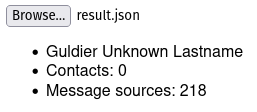
\includegraphics{pmi/img/partialtotal.png}
    \caption{Пример работы при неполных данных}
    \label{fig:dataex}
\end{figure}


При указании некорректных (отсутствующих в данных) пользователей для графа отказа не происходит, такие пользователи фильтруются.

Приложение удовлетворяет требованиям к надежности.